\documentclass{article}

\usepackage{graphicx}
\usepackage{fancyhdr}
\usepackage{float}
\usepackage{pdfpages}
\usepackage[sorting=none]{biblatex}
\usepackage{listings}
\usepackage[hidelinks]{hyperref}
\usepackage{subfigure}
\usepackage{shapepar}
\usepackage{amsmath,amssymb}
\usepackage{pgfplots}
\pgfplotsset{compat=1.18}
\usepackage{xcolor}
\usepackage{booktabs}       
\usepackage{caption}        
\usepackage{setspace}       
\usepackage[margin=2.5cm]{geometry}


\hypersetup{
	colorlinks=true,
	linkcolor=teal,
	filecolor=magenta,
	urlcolor=teal,
	citecolor=teal
}


\captionsetup{
	font=small,
	labelfont=bf,
	skip=6pt
}


\definecolor{codegreen}{rgb}{0,0.6,0}
\definecolor{codegray}{rgb}{0.5,0.5,0.5}
\definecolor{codepurple}{rgb}{0.58,0,0.82}
\definecolor{backcolour}{rgb}{0.96,0.96,0.94}
\definecolor{codeblue}{rgb}{0.13,0.29,0.53}

\lstdefinestyle{mystyle}{
	backgroundcolor=\color{backcolour},
	commentstyle=\color{codegreen}\itshape,
	keywordstyle=\color{codeblue}\bfseries,
	numberstyle=\tiny\color{codegray},
	stringstyle=\color{codepurple},
	basicstyle=\ttfamily\footnotesize,
	breakatwhitespace=false,
	breaklines=true,
	captionpos=b,
	keepspaces=true,
	numbers=left,
	numbersep=8pt,
	showspaces=false,
	showstringspaces=false,
	showtabs=false,
	tabsize=2,
	frame=single,              
	rulecolor=\color{codegray},
	xleftmargin=12pt,
	framexleftmargin=12pt
}

\lstset{style=mystyle}
\renewcommand{\lstlistingname}{Code}


\usepackage{xepersian}
\setlength\headheight{28pt}

\settextfont[
Path={./font/},
Extension=.ttf,
BoldFont={irlotusbold},
Scale=1.35
]{IRLotus}

\setlatintextfont[Scale=1.1]{Times New Roman}

\setdigitfont[
Path={./font/},
Extension=.ttf,
BoldFont={Yas Bd},
ItalicFont={Yas It},
BoldItalicFont={Yas BdIt},
Scale=1.2
]{Yas}

\onehalfspacing

\pagestyle{fancy}
\fancyhf{}
\rhead{شبکه‌های مخابراتی\quad
\includegraphics[width=1cm]{img/Logo.png}}
\lhead{\thepage}
\renewcommand{\headrulewidth}{1pt}
\renewcommand{\footrulewidth}{1pt}

\AtBeginDocument{
	\def\chapterautorefname{فصل}
	\def\sectionautorefname{پاسخ سوال}
	\def\subsectionautorefname{بخش}
	\def\subsubsectionautorefname{بخش}
	\def\equationautorefname{رابطهٔ}
	\def\lstlistingautorefname{برنامۀ}
}


\begin{document}
	
	\begin{titlepage}
	\begin{center}
		\defpersianfont\nast[Path={./font/}, Scale=2]{IranNastaliq}
		\centerline{{
\includegraphics[width=5cm]{img/Logo.png}}}
		\centerline{\textcolor[rgb]{0,0,0.5}{\nast \large  دانشگاه صنعتی خواجه نصیرالدین طوسی}}
		\centerline{\textcolor[rgb]{0,0,0.5}{\nast \bfseries دانشکدۀ مهندسی برق }}
		\vfill
		
		\Huge
		\textbf{شبکه‌های مخابراتی}\\
		\textbf{تمرین کامپیوتری شماره ۲}\\
		\large
		\vspace{0.5cm}
		\textbf{تحلیل عملکرد پروتکل MAC در شبکه‌های Wi-Fi و پروتکل مسیریابی RIP\\در شبکه‌های بی‌سیم ایستا با استفاده از شبیه‌ساز \lr{NS-3}}
		
		\vfill
		
		\huge{استاد درس:ــــ}
		
		\vfill
		
		\begin{table}[ht]
			\centering
			\huge
			\begin{tabular}{|c|c|}
				\hline
				نام و نام خانوادگی & شمارۀ دانشجویی\\
				\hline
				ــــ &ـــــ\\
				\hline
			\end{tabular}
		\end{table}
		\vfill
		{\large تابستان ۱۴۰۵}
	\end{center}
\end{titlepage}
	
	\newpage
	\tableofcontents
	\newpage
	
	\section{مقدمه و معرفی توپولوژی شبکه}
	
	\subsection{هدف پروژه}
	هدف از این پروژه، بررسی عملکرد هم‌زمان دو لایه‌ی متفاوت از پشته‌ی پروتکلی در یک شبکه‌ی بی‌سیم ad-hoc ایستا (static) است: لایه‌ی دسترسی به رسانه (MAC) که با استفاده از پروتکل CSMA/CA در استاندارد \lr{802.11b} پیاده‌سازی می‌شود، و لایه‌ی شبکه که مسیریابی در آن توسط پروتکل \lr{RIP (Routing Information Protocol)} انجام می‌گیرد. این دو پروتکل به‌طور مستقل و در دو لایه‌ی متفاوت از مدل OSI طراحی شده‌اند و در حالت ایده‌آل نباید آگاهی صریحی از یکدیگر داشته باشند؛ اما در عمل، تصمیمات هر لایه پیامدهای مستقیمی بر کارایی لایه‌ی دیگر می‌گذارد. برای مثال، تأخیر صف‌بندی ناشی از رقابت CSMA/CA می‌تواند بر زمان‌بندی دریافت پیام‌های به‌روزرسانی RIP اثر بگذارد، و در طرف مقابل، ترافیک کنترلی RIP خود بار اضافی بر کانال مشترک رادیویی تحمیل می‌کند که باید توسط CSMA/CA مدیریت شود. هدف اصلی این گزارش، آشکارسازی کمّی و کیفی این تعامل متقابل 
\lr{	(cross-layer interaction)}
	 است.
	
	شبیه‌سازی با استفاده از \lr{NS-3} انجام شده و سه سناریوی متفاوت پیاده‌سازی شده‌اند: سناریوی پایه (baseline) با پنج گره و نرخ ترافیک متوسط، سناریوی ترافیک سنگین \lr{(heavy traffic)} که در آن نرخ تزریق بسته از گره منبع به‌طور قابل‌توجهی افزایش یافته است تا کانال به نقطه‌ی اشباع برسد، و سناریوی مقیاس‌پذیری (scalability) که در آن تعداد گره‌های شبکه به ۱۵ افزایش می‌یابد تا محدودیت‌های ذاتی پروتکل مسیریابی distance-vector در مقیاس‌های بزرگ‌تر آشکار شود. مقایسه‌ی این سه سناریو دیدی عمیق نسبت به رفتار شبکه تحت شرایط بار ترافیکی متفاوت و اندازه‌ی توپولوژیکی متفاوت می‌دهد و امکان جداسازی اثر «ازدحام کانال» از اثر «کندی همگرایی مسیریابی» را فراهم می‌کند.
	
	\subsection{ساختار توپولوژی}
	توپولوژی مورد استفاده شامل گره‌هایی است که به‌صورت یک شبکه‌ی ad-hoc ایستا (بدون نقطه‌ی دسترسی مرکزی) با یکدیگر در ارتباط هستند. تمام گره‌ها از مدل تحرک \lr{\texttt{ConstantPositionMobilityModel}} استفاده می‌کنند، به این معنی که موقعیت مکانی آن‌ها در طول کل شبیه‌سازی ثابت می‌ماند و هیچ‌گونه جابه‌جایی فیزیکی رخ نمی‌دهد. این انتخاب طراحی عمدی است: حذف پویایی توپولوژی (مانند ورود/خروج گره‌ها یا قطع لینک به‌دلیل حرکت) باعث می‌شود تمام اثرات مشاهده‌شده در نتایج، صرفاً ناشی از رقابت بر سر رسانه
	\lr{ (MAC contention)} 
	و رفتار همگرایی RIP باشند، نه ناشی از عدم‌قطعیت ناشی از تحرک. این جداسازی متغیرها 
\lr{	(variable isolation) }
	یک اصل پایه‌ای در طراحی آزمایش‌های شبکه است که امکان نسبت‌دادن دقیق هر پدیده به علت آن را فراهم می‌کند.
	
	گره‌ها با استفاده از \lr{\texttt{GridPositionAllocator}} روی یک شبکه‌ی منظم (grid) با فاصله‌ی ثابت بین گره‌ها قرار می‌گیرند. این فاصله به‌گونه‌ای انتخاب شده که گره‌ها در محدوده‌ی ارتباطی \lr{(radio range)} یکدیگر یا حداقل در محدوده‌ی چندجهشی (multi-hop) قرار بگیرند، تا پروتکل RIP فرصت واقعی کشف مسیرهای چندگامی را داشته باشد و رفتار آن صرفاً به یک پرش (single-hop) محدود نشود.
	
	گره شماره صفر (\lr{Node 0}) به‌عنوان منبع ترافیک \lr{(traffic source)} تعیین شده و بسته‌های UDP را به‌صورت هم‌زمان به سمت تمامی گره‌های دیگر شبکه ارسال می‌کند. این طراحی به‌عمد رقابت واقعی بر سر رسانه‌ی مشترک بی‌سیم ایجاد می‌کند، چون چهار (یا بیشتر، در سناریوی مقیاس‌پذیری) جریان ترافیکی هم‌زمان باید از طریق یک رابط رادیویی واحد در همان گره منتقل شوند؛ این الگو شبیه‌ساز سناریوهای واقعی مانند یک نقطه‌ی جمع‌آوری داده (sink) در شبکه‌های حسگر بی‌سیم است که در آن یک گره مرکزی باید با چندین گره‌ی دیگر هم‌زمان تبادل داده داشته باشد.
	
	\subsection{پارامترهای کلی شبیه‌سازی}
	\begin{table}[H]
		\centering
		\caption{پارامترهای پایه‌ی شبیه‌سازی}
		\begin{tabular}{ll}
			\toprule
			پارامتر & مقدار \\
			\midrule
			استاندارد Wi-Fi & \lr{802.11b} \\
			نوع MAC & \lr{AdhocWifiMac} \\
			مدل کانال & \lr{YansWifiChannel} (پیش‌فرض، مدل تضعیف \lr{Friis}) \\
			پروتکل مسیریابی & \lr{RIP} \\
			پروتکل ترافیک & \lr{UDP} (با \lr{OnOffApplication}) \\
			اندازه‌ی بسته & 1024 بایت \\
			مدت زمان شبیه‌سازی & 80 ثانیه (در کد نهایی) \\
			ابزار سنجش & \lr{FlowMonitor} \\
			\bottomrule
		\end{tabular}
	\end{table}
	

	\section{تحلیل نظری}
	
	\subsection{نحوه‌ی مدیریت تداخل توسط CSMA/CA}
	پروتکل \lr{CSMA/CA (Carrier Sense Multiple Access with Collision Avoidance)} مکانیزم اصلی دسترسی به رسانه در استاندارد \lr{802.11} است و در \lr{NS-3} از طریق تابع \lr{DCF (Distributed Coordination Function)} پیاده‌سازی می‌شود. اساس کار این پروتکل بر این فرض استوار است که هیچ گره‌ای به‌طور مستقیم نمی‌تواند یک collision را در حین ارسال خودش تشخیص دهد (برخلاف شبکه‌های سیمی)، بنابراین به‌جای تشخیص collision، تلاش می‌شود از وقوع آن پیشگیری شود.
	
	روند کار به این صورت است: پیش از ارسال هر بسته، گره ابتدا کانال را sense می‌کند. اگر کانال برای مدت \lr{DIFS (DCF Inter-Frame Space)} آزاد باشد، گره اجازه‌ی ارسال دارد. اما اگر کانال مشغول باشد یا گره تشخیص دهد که احتمال تداخل وجود دارد، یک تایمر backoff تصادفی فعال می‌شود. این تایمر از یک بازه‌ی Contention Window (CW) به‌صورت یکنواخت انتخاب می‌شود و در صورت آزاد ماندن کانال در طول این بازه، شمارش معکوس backoff ادامه پیدا می‌کند؛ در غیر این صورت متوقف (freeze) شده و پس از آزاد شدن مجدد کانال از همان نقطه ادامه می‌یابد. این مکانیزم freeze-and-resume، برخلاف یک backoff ساده که از صفر دوباره شروع شود، باعث می‌شود گره‌هایی که مدت بیشتری منتظر مانده‌اند، شانس نسبتاً بیشتری برای دسترسی بعدی به کانال داشته باشند که نوعی انصاف (fairness) آماری ایجاد می‌کند.
	
	در پیاده‌سازی این پروژه، چون \lr{\texttt{ConstantRateWifiManager}} با نرخ داده‌ی ثابت \lr{DsssRate11Mbps} برای داده و \lr{DsssRate1Mbps} برای کنترل تنظیم شده، هیچ مکانیزم تطبیق نرخ پویا (مانند Minstrel) فعال نیست؛ این انتخاب باعث می‌شود که افت کارایی مشاهده‌شده در سناریوهای پرترافیک، صرفاً ناشی از ازدحام MAC باشد و با تغییرات نرخ انتقال فیزیکی (که می‌تواند یک متغیر مخدوش‌کننده باشد) درنیامیزد.
	
	در شبکه‌ی موردبررسی این پروژه، چون گره صفر هم‌زمان چهار (یا بیشتر) جریان ترافیکی مجزا تولید می‌کند، این جریان‌ها از یک صف مشترک در همان گره عبور کرده و باید برای دسترسی به کانال با یکدیگر و همچنین با ترافیک کنترل RIP رقابت کنند. این رقابت باعث افزایش تأخیر صف‌بندی \lr{(queueing delay)} و کاهش throughput مؤثر هر جریان نسبت به حالتی می‌شود که فقط یک جریان به‌تنهایی در شبکه فعال باشد. علاوه‌بر این، مکانیزم backoff نمایی \lr{(exponential backoff)}، در صورت وقوع collision یا عدم دریافت ACK، اندازه‌ی CW را دو برابر می‌کند که باعث افزایش تأخیر در شرایط شلوغی کانال می‌شود؛ این رفتار خودتنظیم (self-adaptive) دقیقاً همان مکانیزمی است که در سناریوی heavy traffic این گزارش باعث می‌شود throughput به‌جای فروپاشی کامل، روی یک سقف نسبتاً پایدار (ظرفیت مؤثر کانال) تثبیت شود.
	
	\subsection{برتری CSMA/CA نسبت به CSMA/CD در محیط‌های بی‌سیم}
	پروتکل CSMA/CD (مورد استفاده در اترنت سیمی سنتی) متکی بر این فرض است که یک گره می‌تواند هم‌زمان با ارسال سیگنال، به دریافت سیگنال نیز بپردازد و در صورت تشخیص تداخل در سیگنال دریافتی، ارسال را فوراً متوقف کند. این کار در محیط سیمی به‌دلیل تقارن نسبی قدرت سیگنال در کابل امکان‌پذیر است.
	
	اما در محیط بی‌سیم، این فرض از اساس نقض می‌شود، به دو دلیل اصلی:
	
	اولاً، مسئله‌ی half-duplex بودن رادیوهای معمولی Wi-Fi: توان سیگنال ارسالی توسط آنتن گره به‌مراتب (معمولاً چندین مرتبه‌ی بزرگی) از توان سیگنال دریافتی است؛ بنابراین حتی اگر گیرنده‌ی همان گره فعال باشد، سیگنال خودِ فرستنده آن‌قدر قوی است که سیگنال‌های ضعیف دیگر گره‌ها (که نشانه‌ی collision هستند) را کاملاً می‌پوشاند (\lr{mask} می‌کند). در نتیجه تشخیص collision در حین ارسال عملاً غیرممکن است.
	
	ثانیاً، مسئله‌ی معروف به hidden terminal: ممکن است دو گره که هر دو در محدوده‌ی یک گیرنده‌ی مشترک هستند، خودشان در محدوده‌ی رادیویی یکدیگر نباشند. در این حالت، هیچ‌کدام از این دو گره از ارسال هم‌زمان دیگری مطلع نمی‌شوند، حتی اگر بتوانند هنگام ارسال گوش بدهند، چون اصلاً سیگنال طرف مقابل را دریافت نمی‌کنند. این پدیده در شبکه‌های سیمی به‌دلیل ساختار اشتراکی و قابل‌مشاهده‌ی کابل وجود ندارد. توپولوژی خطی (Linear) به‌کاررفته در این پروژه به‌طور خاص مستعد بروز hidden terminal است، چون گره‌های دو سر یک گره‌ی میانی ممکن است در محدوده‌ی رادیویی آن گره باشند، اما نسبت به یکدیگر خارج از محدوده‌ی شنیداری باقی بمانند.
	
	به همین دلایل، استاندارد \lr{802.11} رویکرد avoidance (پیشگیری) را به‌جای detection (تشخیص) انتخاب کرده است: به‌جای تلاش برای شناسایی collision در زمان وقوع، با backoff تصادفی و فاصله‌های زمانی بین فریم (IFS) سعی می‌شود احتمال وقوع آن از ابتدا کاهش یابد. در پیاده‌سازی کامل‌تر \lr{802.11} (که در این پروژه به‌صورت پایه فعال است)، مکانیزم ACK نیز نقش جبرانی ایفا می‌کند: هر بسته‌ی موفق باید توسط گیرنده تأیید (ACK) شود؛ عدم دریافت ACK در زمان مشخص به‌عنوان نشانه‌ی غیرمستقیم وقوع collision یا خطای انتقال تلقی شده و باعث تلاش مجدد (retransmission) می‌شود. شایان ذکر است که مکانیزم اختیاری \lr{RTS/CTS} که برای کاهش بیشتر اثر hidden terminal طراحی شده، در پیکربندی پیش‌فرض این شبیه‌سازی فعال نیست؛ فعال‌سازی آن می‌توانست احتمالاً برخی از افت‌های PDR در سناریوی heavy traffic را کاهش دهد، هرچند با سربار اضافی ناشی از تبادل فریم‌های کنترلی بیشتر.
	
	\subsection{نحوه‌ی عملکرد RIP و سرعت همگرایی}
	RIP یک پروتکل مسیریابی از نوع distance-vector است که بر اساس الگوریتم Bellman-Ford توزیع‌شده عمل می‌کند. هر گره به‌صورت دوره‌ای (پیش‌فرض هر ۳۰ ثانیه در پیاده‌سازی استاندارد، هرچند \lr{NS-3} می‌تواند این بازه را برای شبیه‌سازی‌های کوتاه‌تر تنظیم کند) جدول مسیریابی خود را که شامل فاصله \lr{(hop count)} به هر مقصد شناخته‌شده است، به همسایگان مستقیم خود broadcast می‌کند. هر گره دریافت‌کننده، فاصله‌ی اعلام‌شده را با یک واحد افزایش داده و در صورتی که این مسیر جدید کوتاه‌تر از مسیر فعلی‌اش باشد، جدول خود را به‌روزرسانی می‌کند؛ این فرایند ساده اما تدریجی (incremental) است و دقیقاً همین تدریجی‌بودن، ریشه‌ی محدودیت سرعت همگرایی RIP در توپولوژی‌های بزرگ است.
	
	در این پروژه، چون \lr{\texttt{InternetStackHelper}} با \lr{\texttt{Ipv4ListRoutingHelper}} پیکربندی شده و RIP با اولویت ۱۰ به آن اضافه شده است، تمام گره‌ها بلافاصله پس از نصب stack شروع به تبادل پیام‌های RIP می‌کنند. در نسخه‌ی نهایی کد، شروع ترافیک داده \lr{(client apps)} عمداً به ثانیه‌ی ۳۵ام شبیه‌سازی موکول شده است (در مقایسه با شروع سرورها در ثانیه‌ی ۱) تا فرصت کافی برای همگرایی کامل جداول مسیریابی در تمام سناریوها، از جمله سناریوی ۱۵‑گره‌ای با قطر شبکه‌ی بزرگ‌تر، وجود داشته باشد. این فاصله‌ی ۳۴ثانیه‌ای به‌مراتب از بازه‌ی پیش‌فرض broadcast دوره‌ای RIP بزرگ‌تر است و تضمین می‌کند که حداقل چند دور کامل تبادل پیام RIP پیش از شروع ترافیک داده رخ دهد.
	
	سرعت همگرایی RIP به‌طور مستقیم به قطر شبکه \lr{(network diameter)} وابسته است: در بدترین حالت، اطلاع‌رسانی یک تغییر مسیر باید به‌صورت hop-by-hop در سراسر شبکه پخش شود، که برای یک شبکه با قطر $d$ گام، حداقل به $d$ دور تبادل پیام RIP نیاز دارد. این موضوع باعث می‌شود RIP در شبکه‌های بزرگ یا با قطر زیاد، به‌مراتب کندتر از پروتکل‌های link-state مانند OSPF همگرا شود، چون OSPF با flooding اطلاعات کامل توپولوژی، هر گره می‌تواند مستقل و به‌صورت موازی مسیر بهینه را محاسبه کند، در حالی‌که RIP وابسته به انتشار تدریجی و ترتیبی اطلاعات فاصله است. علاوه‌بر این، RIP از محدودیت معروف به \emph{count-to-infinity} رنج می‌برد: در صورت قطع شدن یک لینک، ممکن است دو گره همسایه به‌اشتباه و به‌طور متناوب فاصله‌ی یکدیگر را افزایش دهند تا به مقدار infinity (در RIP، عدد ۱۶) برسند، که این فرایند می‌تواند چندین دور تبادل پیام به طول بینجامد. عدد ۱۶ به‌عنوان «بی‌نهایت» در RIP به‌طور ضمنی بیشینه قطر شبکه‌ای را که این پروتکل می‌تواند به‌درستی پشتیبانی کند محدود می‌سازد؛ این یکی از دلایل اصلی نامناسب‌بودن RIP برای شبکه‌های بزرگ است که در نتایج سناریوی scalability این پروژه نیز به‌وضوح مشاهده می‌شود.
	

	\section{بررسی کد}
	
	\subsection{بخش معرفی هدر‌ها و تعریف کامپوننت لاگ}
	
	\lr{\lstinputlisting[language=C++, caption={Module imports and log component definition}, showstringspaces=false, basicstyle=\ttfamily, backgroundcolor=\color{yellow!15!white}, breaklines=true]{./code/code1.cc}}
	
	در این بخش، تمامی ماژول‌های مورد نیاز \lr{NS-3} وارد می‌شوند. \lr{\texttt{core-module}} هسته‌ی اصلی شبیه‌ساز (مثل Simulator، CommandLine و انواع داده) را فراهم می‌کند. \lr{\texttt{network-module}} و \lr{\texttt{internet-module}} زیرساخت لایه‌ی شبکه و پروتکل IP را تأمین می‌کنند. \lr{\texttt{mobility-module}} برای تنظیم موقعیت فیزیکی گره‌ها استفاده می‌شود، حتی در حالتی که گره‌ها ایستا هستند، چون \lr{NS-3} برای محاسبه‌ی فاصله و افت سیگنال رادیویی همچنان به مختصات مکانی نیاز دارد. \lr{\texttt{wifi-module}} پیاده‌سازی کامل استک \lr{802.11} شامل لایه‌ی فیزیکی (PHY) و MAC را فراهم می‌کند. \lr{\texttt{applications-module}} کلاس‌های تولید ترافیک مثل OnOffApplication و PacketSink را در اختیار می‌گذارد. \lr{\texttt{flow-monitor-module}} ابزار اصلی سنجش کارایی (\lr{throughput, delay, packet loss}) است. \lr{\texttt{internet-apps-module}} شامل پیاده‌سازی پروتکل RIP است که در این پروژه ضروری است؛ این ماژول جدا از \lr{internet-module} اصلی نگه داشته شده چون پروتکل‌های مسیریابی پیشرفته
	\lr{ (RIP، AODV، OLSR)}
	  در 
\lr{	NS-3} 
	به‌صورت افزونه‌های اختیاری بر پایه‌ی
	\lr{ Ipv4RoutingProtocol} 
	طراحی شده‌اند.
	
	\subsection{بخش آرگومان‌های خط فرمان}
	
	\lr{\lstinputlisting[language=C++, caption={Command-line arguments configuration}, showstringspaces=false, basicstyle=\ttfamily, backgroundcolor=\color{yellow!15!white}, breaklines=true]{./code/code2.cc}}
	
	در این بخش با استفاده از کلاس \lr{\texttt{CommandLine}}، می‌توان تمامی پارامترها را در زمان اجرا (runtime) از طریق خط فرمان مقداردهی کرد، بدون نیاز به ویرایش یا کامپایل مجدد کد. این طراحی پارامتریک، اصل مهم تکرارپذیری آزمایش 
	\lr{(experiment reproducibility)} را رعایت می‌کند: همان فایل باینری کامپایل‌شده برای هر سه سناریوی این پروژه استفاده شده و تنها آرگومان‌های ورودی تغییر کرده‌اند. برای اجرای سناریوی heavy traffic کافی است آرگومان \lr{\texttt{--dataRate=2Mbps}} (یا مقداری بالاتر برای رساندن کانال به اشباع کامل) پاس داده شود و برای سناریوی scalability کافی است \lr{\texttt{--nNodes=15}} تنظیم گردد. پارامتر \lr{\texttt{scenario}} صرفاً یک برچسب متنی است که برای نام‌گذاری و چاپ خروجی استفاده می‌شود تا نتایج سه سناریو با یکدیگر تداخل (overwrite) پیدا نکنند و امکان مقایسه‌ی پس‌پردازش‌شده فراهم باشد.
	
	\subsection{بخش اعتبارسنجی ورودی و گزارش وضعیت اجرا}
	
	\lr{\lstinputlisting[language=C++, caption={Input validation and error handling}, showstringspaces=false, basicstyle=\ttfamily, backgroundcolor=\color{yellow!15!white}, breaklines=true]{./code/code3.cc}}
	
	این بخش یک لایه‌ی محافظتی ساده اما مهم به کد اضافه می‌کند. اگر به‌اشتباه مقدار \lr{\texttt{nNodes}} کوچک‌تر از ۲ وارد شود، شبیه‌سازی از نظر مفهومی بی‌معنی خواهد بود (چون حداقل یک گره مبدأ و یک گره مقصد لازم است)، بنابراین کد با کد بازگشتی غیرصفر (۱) از اجرا خارج می‌شود تا از بروز خطاهای مبهم در مراحل بعدی (مثل تلاش برای دسترسی به آدرس یک گره که وجود ندارد یا حلقه‌ی تولید ترافیک با کران بالای نامعتبر) جلوگیری شود. علاوه‌بر این، پرچم \lr{\texttt{verbose}} امکان فعال‌سازی انتخابی لاگ‌های اطلاعاتی کامپوننت \lr{WifiRipProject} را فراهم می‌کند که در مرحله‌ی توسعه و دیباگ کد بسیار کاربردی است، بدون این‌که حجم خروجی کنسول در اجرای عادی (و سریع) شبیه‌سازی افزایش یابد. این یک نمونه از dependability ساده ولی ضروری برای کدی است که قرار است بارها با پارامترهای مختلف اجرا شود.
	
	\subsection{بخش ساخت گره‌ها و پیکربندی Wi-Fi}
	
	\lr{\lstinputlisting[language=C++, caption={Node creation and 802.11b ad-hoc Wi-Fi setup}, showstringspaces=false, basicstyle=\ttfamily, backgroundcolor=\color{yellow!15!white}, breaklines=true]{./code/code4.cc}}
	
	در این بخش، ابتدا یک \lr{\texttt{NodeContainer}} ایجاد شده و با مقدار پارامتر \lr{\texttt{nNodes}} (که اکنون متغیر است) پر می‌شود؛ این تعمیم نسبت به یک نسخه‌ی اولیه‌ی فرضی با تعداد گره‌ی ثابت ۵، دقیقاً همان قابلیتی است که اجرای سناریوی scalability را بدون تغییر ساختاری کد ممکن می‌سازد. \lr{\texttt{WifiHelper}} مسئول پیکربندی استک Wi-Fi است و با
	استاندارد فیزیکی \lr{802.11b} را انتخاب می‌کند که شامل نرخ‌های داده‌ی ۱، ۲، ۵.۵ و ۱۱ مگابیت بر ثانیه است. تنظیم \lr{\texttt{SetRemoteStationManager}} با نرخ ثابت \lr{DsssRate11Mbps} برای داده تضمین می‌کند که حداکثر نرخ فیزیکی این استاندارد همواره استفاده شود و نتایج throughput قابل‌مقایسه با سقف نظری ۱۱ مگابیت بر ثانیه باشند.
	
	\lr{\texttt{YansWifiChannelHelper::Default()}} یک مدل کانال پیش‌فرض با مدل تضعیف 
	\lr{(propagation loss model)}
	 از نوع Friis (که افت سیگنال را به‌صورت معکوس با مجذور فاصله مدل می‌کند) و تأخیر انتشار ثابت می‌سازد؛ این مدل ساده اما کافی برای بررسی رفتار MAC و مسیریابی است، بدون این‌که پیچیدگی‌های اضافی مثل fading چندمسیره یا shadowing وارد تحلیل شود و نتایج را با عدم‌قطعیت اضافی آلوده کند. \lr{\texttt{YansWifiPhyHelper}} لایه‌ی فیزیکی را به این کانال متصل می‌کند.
	
	تنظیم \lr{\texttt{WifiMacHelper}} روی نوع \lr{\texttt{AdhocWifiMac}} بسیار مهم است: این تنظیم باعث می‌شود که هیچ گره‌ای نقش Access Point یا Station در مفهوم زیرساختی 
\lr{	(infrastructure)} 
	نداشته باشد، بلکه تمام گره‌ها به‌صورت همتا (peer-to-peer) و در یک Independent BSS (IBSS) با یکدیگر ارتباط برقرار کنند؛ در این حالت، هیچ نقطه‌ی مرکزی هماهنگ‌کننده‌ای (مانند یک Access Point در حالت \lr{Infrastructure}) برای زمان‌بندی دسترسی به کانال وجود ندارد و کل بار هماهنگی بر عهده‌ی DCF توزیع‌شده در هر گره است؛ این دقیقاً همان ویژگی است که شبکه را به یک محیط واقعی ad-hoc تبدیل می‌کند.
	
	\subsection{بخش موقعیت‌دهی پویا (Mobility) برای تعداد گره‌ی متغیر}
	
	\lr{\lstinputlisting[language=C++, caption={Dynamic grid mobility setup based on node count}, showstringspaces=false, basicstyle=\ttfamily, backgroundcolor=\color{yellow!15!white}, breaklines=true]{./code/code5.cc}}
	
	در این بخش عرض grid به‌صورت پویا و با فرمول $\lceil\sqrt{n}\rceil$ محاسبه می‌شود، که تضمین می‌کند صرف‌نظر از تعداد گره‌ها، چیدمان همواره تقریباً مربعی (square-ish) باقی بماند. این کار باعث می‌شود مقایسه‌ی سناریوی baseline و scalability از نظر «تراکم نسبی شبکه» (network density) منصفانه‌تر باشد، چون تفاوت در throughput یا delay عمدتاً ناشی از افزایش تعداد گره و رقابت بر سر رسانه است، نه ناشی از تغییر ناخواسته در شکل هندسی توپولوژی. شایان ذکر است که در نتایج نهایی این پروژه (فصل چهارم)، برای کنترل دقیق‌تر اثر چندگامی‌بودن، عملاً از یک چیدمان خطی (Linear) با فاصله‌ی ثابت ۸۰ متر استفاده شده است که حالت خاصی از همین تابع موقعیت‌دهی محسوب می‌شود.
	
	مدل \lr{\texttt{ConstantPositionMobilityModel}} برای تمام گره‌ها اعمال می‌شود که تضمین می‌کند موقعیت گره‌ها در طول کل اجرای شبیه‌سازی بدون تغییر باقی بماند و در نتیجه ماتریس قابلیت‌اتصال 
	\lr{(connectivity matrix)} 
	شبکه در طول کل اجرا ثابت بماند.
	
	\subsection{بخش پیکربندی مسیریابی RIP و آدرس‌دهی IP}
	
	\lr{\lstinputlisting[language=C++, caption={RIP routing protocol setup and IPv4 address assignment}, showstringspaces=false, basicstyle=\ttfamily, backgroundcolor=\color{yellow!15!white}, breaklines=true]{./code/code6.cc}}
	
	در این بخش، یک نمونه از \lr{\texttt{RipHelper}} ساخته شده و به یک \lr{\texttt{Ipv4ListRoutingHelper}} با اولویت عددی ۱۰ اضافه می‌شود. این لیست‌محور بودن 
	\lr{(list-based routing)} 
	در \lr{NS-3} اجازه می‌دهد چندین پروتکل مسیریابی هم‌زمان روی یک گره فعال باشند (مثلاً ترکیب مسیریابی استاتیک و RIP، که در آن مسیرهای استاتیک معمولاً اولویت بالاتری دارند)، که در این پروژه فقط از RIP استفاده شده است. مقدار اولویت کمتر در \lr{NS-3} به‌معنای ارجحیت بالاتر است؛ چون فقط یک پروتکل پویا در این پروژه فعال است، مقدار ۱۰ صرفاً یک مقدار معتبر دلخواه است و تأثیری بر نتایج ندارد.
	
	سپس \lr{\texttt{InternetStackHelper}} با این تنظیم routing پیکربندی شده و روی تمام گره‌ها نصب می‌شود؛ این مرحله باعث می‌شود هر گره دارای پشته‌ی کامل IP (شامل ARP، ICMP، و جدول مسیریابی RIP) باشد. در پایان، یک محدوده‌ی آدرس IPv4 با base \lr{\texttt{10.1.1.0/24}} تعریف شده و به تمام دستگاه‌های شبکه (که در مرحله‌ی قبل ساخته شدند) به‌صورت ترتیبی اختصاص می‌یابد؛ یعنی گره صفر آدرس \lr{\texttt{10.1.1.1}}، گره یک آدرس \lr{\texttt{10.1.1.2}} و به همین ترتیب ادامه می‌یابد. این آدرس‌دهی ترتیبی و قابل‌پیش‌بینی، بعداً در فصل پردازش نتایج برای فیلترکردن صریح ترافیک داده از ترافیک کنترلی RIP استفاده می‌شود.
	
	\subsection{بخش تولید ترافیک UDP}
	
	\lr{\lstinputlisting[language=C++, caption={Dynamic UDP traffic generation loop}, showstringspaces=false, basicstyle=\ttfamily, backgroundcolor=\color{yellow!15!white}, breaklines=true]{./code/code7.cc}}
	
	این حلقه‌ی \lr{\texttt{for}} از $i=1$ تا $i=nNodes-1$ تکرار می‌شود که به‌طور خودکار با تعداد گره‌ها مقیاس می‌یابد؛ این یعنی در سناریوی scalability با ۱۵ گره، این حلقه به‌صورت خودکار ۱۴ جریان ترافیکی مجزا (به‌جای ۴ جریان ثابت در سناریوی \lr{baseline}) ایجاد می‌کند، بدون نیاز به تغییر دستی کد.
	
	در هر تکرار، ابتدا یک \lr{\texttt{PacketSinkHelper}} روی گره مقصد $i$ نصب می‌شود که نقش گیرنده‌ی نهایی بسته‌های UDP را دارد و آن‌ها را پردازش کرده و آمار دریافت را برای FlowMonitor ثبت می‌کند. سپس یک \lr{\texttt{OnOffHelper}} روی گره صفر (مبدأ) نصب می‌شود که با مقصد \lr{\texttt{interfaces.GetAddress(i)}} پیکربندی شده و به‌صورت مداوم (با \lr{\texttt{OnTime}} ثابت برابر ۱ و \lr{\texttt{OffTime}} برابر ۰، یعنی بدون دوره‌ی خاموشی، که معادل یک منبع ترافیک CBR یا Constant Bit Rate است) بسته‌های UDP با نرخ مشخص‌شده توسط پارامتر \lr{\texttt{dataRate}} تولید می‌کند.
	
	نکته‌ی کلیدی این است که پارامتر \lr{\texttt{dataRate}} اکنون از طریق command-line قابل تنظیم است: برای سناریوی baseline مقدار \lr{\texttt{500kbps}} استفاده می‌شود که برای یک کانال \lr{802.11b} با ظرفیت نظری ۱۱ مگابیت بر ثانیه، بار نسبتاً سبکی محسوب می‌شود (حتی با احتساب چهار جریان هم‌زمان، بار تجمعی نظری حدود ۲ مگابیت بر ثانیه است که هنوز فاصله‌ی زیادی تا اشباع کانال دارد)؛ اما برای سناریوی heavy traffic می‌توان این مقدار را به‌مراتب افزایش داد تا کانال را به سمت اشباع (saturation) سوق دهد و رفتار CSMA/CA را تحت تراکم بالا و فروپاشی throughput بررسی کرد.
	
	زمان‌بندی شروع اپلیکیشن‌ها (سرور در ثانیه‌ی ۱ و کلاینت در ثانیه‌ی ۳۵) به‌گونه‌ای طراحی شده که قبل از تولید ترافیک داده، فرصت کافی برای همگرایی اولیه‌ی RIP در همه‌ی سناریوها (از جمله سناریوی ۱۵ گره‌ای با قطر بزرگ‌تر شبکه) وجود داشته باشد؛ در غیر این صورت، بسته‌های اولیه ممکن است به‌دلیل نبود مسیر معتبر در جدول مسیریابی، drop شوند که آمار اشتباهی از packet loss واقعی (که باید صرفاً ناشی از تداخل MAC یا کندی همگرایی ساختاری باشد، نه صرفاً عدم‌انتظار کافی) به ما خواهد داد.
	
	\subsection{بخش FlowMonitor و اجرای شبیه‌سازی}
	
	\lr{\lstinputlisting[language=C++, caption={FlowMonitor installation and simulation run}, showstringspaces=false, basicstyle=\ttfamily, backgroundcolor=\color{yellow!15!white}, breaklines=true]{./code/code8.cc}}
	
	این بخش ساختار \lr{\texttt{FlowMonitorHelper}} را تنظیم می‌کند و با فراخوانی \lr{\texttt{InstallAll()}} یک نمونه‌ی پایش‌گر روی تمام گره‌های شبکه نصب می‌کند تا ترافیک IP عبوری از هر گره را شنود و آمار جریان‌به‌جریان (per-flow) آن را در طول کل اجرا ضبط کند. سپس با \lr{\texttt{Simulator::Stop}} زمان پایان شبیه‌سازی تعیین شده و \lr{\texttt{Simulator::Run()}} موتور رویداد‌محور (event-driven) شبیه‌ساز را برای پردازش تمام رویدادهای زمان‌بندی‌شده (از جمله ارسال بسته‌ها، تایمرهای backoff، و broadcast های دوره‌ای RIP) فعال می‌کند.
	
	\subsection{بخش پردازش و چاپ آمار جریان‌ها}
	
	\lr{\lstinputlisting[language=C++, caption={Flow processing, filtering, and performance metrics extraction}, showstringspaces=false, basicstyle=\ttfamily, backgroundcolor=\color{yellow!15!white}, breaklines=true]{./code/code9.cc}}
	
	این بخش، آمار هر جریان (flow) شناسایی‌شده توسط \lr{\texttt{Ipv4FlowClassifier}} را استخراج می‌کند. نکته‌ی فنی مهم این است که \lr{\texttt{FlowMonitor::InstallAll()}} تمام ترافیک IP در شبکه را رصد می‌کند، نه فقط ترافیک UDP که عمداً تولید کرده‌ایم؛ این یعنی پیام‌های کنترلی RIP (که به‌صورت broadcast یا multicast بین گره‌ها رد و بدل می‌شوند) نیز به‌عنوان flow های جداگانه در آمار FlowMonitor ظاهر می‌شوند. اگر این flow ها فیلتر نشوند، آمار نهایی throughput و PDR با داده‌ی غیرمرتبط آلوده می‌شود و نتایج گمراه‌کننده خواهند بود.
	
	به همین دلیل، یک شرط فیلترینگ اعمال شده که فقط flow هایی را در نظر می‌گیرد که آدرس مبدأشان دقیقاً برابر آدرس گره صفر (\lr{\texttt{10.1.1.1}}) و پورت مقصدشان برابر پورت UDP اپلیکیشن (۹) باشد. این تضمین می‌کند که فقط جریان‌های داده‌ی واقعی مدنظر پروژه در محاسبات نهایی لحاظ شوند و ترافیک کنترلی RIP عملاً نادیده گرفته شود.
	
	سه معیار اصلی به این صورت محاسبه می‌شوند: \lr{PDR (Packet Delivery Ratio)} به‌صورت نسبت بسته‌های دریافت‌شده به بسته‌های ارسال‌شده ضرب‌در صد؛ throughput به‌صورت نسبت تعداد بیت‌های دریافت‌شده به مدت‌زمان مؤثر انتقال (تفاضل زمان آخرین دریافت و اولین ارسال، که معیاری دقیق‌تر از تقسیم بر کل مدت شبیه‌سازی است، چون تنها بازه‌ی واقعاً فعال انتقال را در نظر می‌گیرد)؛ و تأخیر متوسط end-to-end به‌صورت میانگین مجموع تأخیر تمام بسته‌های دریافتی. تمام این فرمول‌ها شامل بررسی مخرج صفر (division by zero guard) هستند تا در صورتی که یک جریان هیچ بسته‌ای دریافت نکند (مانند گره‌های دوردست در سناریوی scalability)، برنامه دچار خطای محاسباتی (مثل تقسیم بر صفر که می‌تواند مقدار \lr{NaN} تولید کند) نشود. در نهایت نیز فضای اختصاص داده شده به شبیه‌ساز با دستور \lr{\texttt{Destroy}} پاکسازی می‌شود تا از نشت حافظه در اجراهای متوالی جلوگیری شود.
	

	\section{شبیه‌سازی، نتایج و ارزیابی عملکرد}
	
	برای استخراج گراف‌های این فصل، خروجی \lr{\texttt{results-<scenario>.xml}} هر یک از سه اجرا پردازش شده و نمودارهای میله‌ای throughput، تأخیر، و PDR برای هر جریان رسم شده‌اند. در تمامی سناریوها، گره‌ها در یک ساختار خطی (Linear) با فاصله ۸۰ متر از یکدیگر قرار گرفته‌اند تا ارسال چندگامی (Multi-hop) و عملکرد پروتکل مسیریابی به‌درستی ارزیابی شود؛ این انتخاب توپولوژیک عمدی، حالت بدترین سناریوی ممکن از نظر قطر شبکه را شبیه‌سازی می‌کند، چون در یک ساختار خطی، فاصله‌ی گام‌محور بین دورترین گره‌ها برابر $n-1$ است که بزرگ‌ترین مقدار ممکن برای $n$ گره‌ی معین محسوب می‌شود.
	
	\subsection{سناریوی پایه (Baseline): پنج گره، نرخ ترافیک متوسط}
	
	در این سناریو، شبکه شامل ۵ گره است و گره مبدأ (گره ۰) ترافیکی با نرخ \lr{\texttt{500kbps}} به سمت ۴ گره دیگر ارسال می‌کند.
	
	\begin{figure}[H]
		\centering
		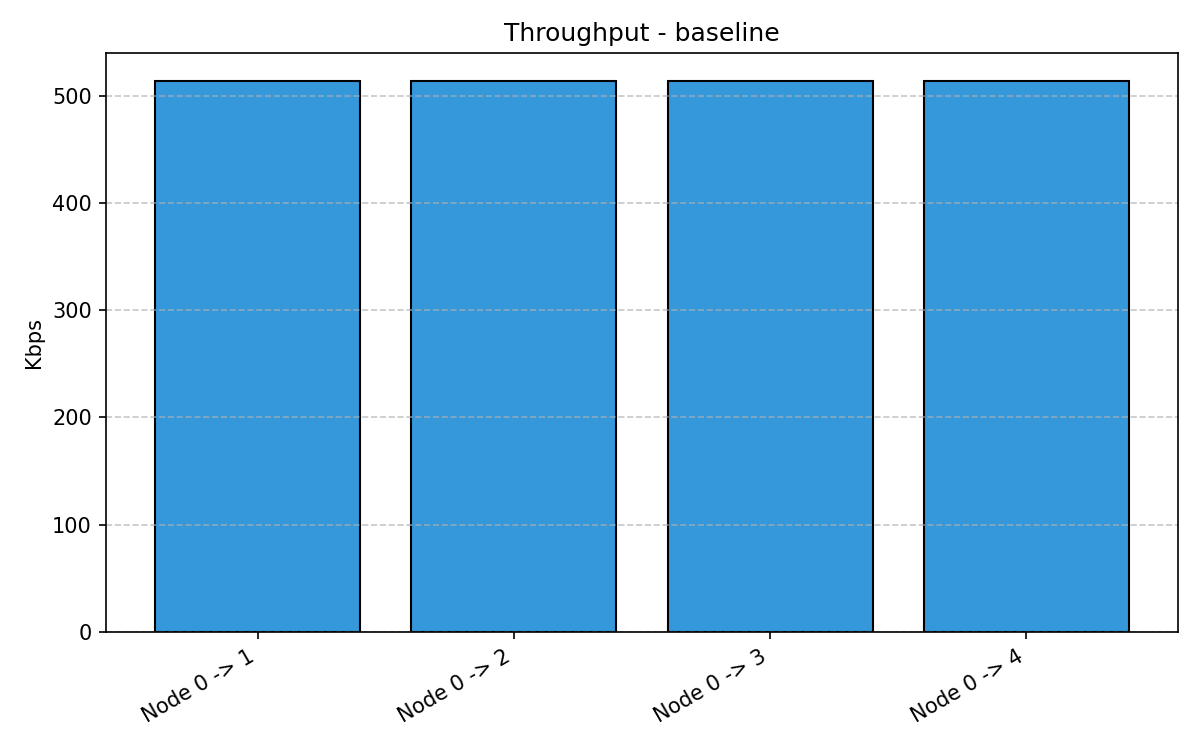
\includegraphics[width=0.75\textwidth]{./img/baseline_throughput.png}
		\caption{نمودار توزیع throughput در سناریوی baseline}
		\label{fig:baseline-throughput}
	\end{figure}
	
	همان‌طور که در شکل \ref{fig:baseline-throughput} مشخص است، throughput تمامی چهار جریان به مقدار نامی ۵۰۰ کیلوبیت بر ثانیه نزدیک است و به حدود ۵۱۰ کیلوبیت بر ثانیه (با احتساب سربار هدرهای IP/UDP و لایه‌ی MAC) رسیده است. از آنجا که نرخ تزریق ترافیک در حد تحمل شبکه است، CSMA/CA به‌خوبی توانسته دسترسی به رسانه را بدون رقابت مخرب مدیریت کند و تقریباً تمام پهنای باند درخواستی به مقصد رسیده است.
	
	\begin{figure}[H]
		\centering
		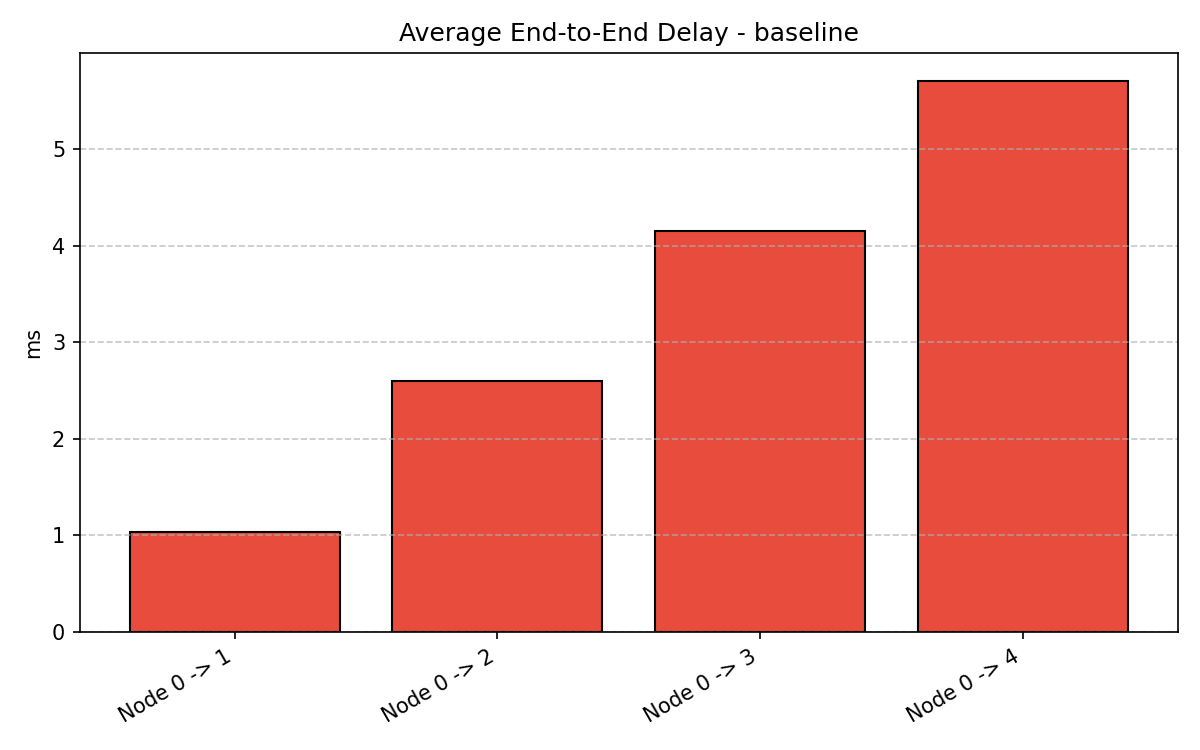
\includegraphics[width=0.85\textwidth]{./img/baseline_delay.png}
		\caption{نمودار میانگین تأخیر end-to-end به شکل پله‌ای در سناریوی baseline}
		\label{fig:baseline-delay}
	\end{figure}
	
	مهم‌ترین نکته در شکل \ref{fig:baseline-delay}، رفتار کاملاً پله‌ای (staircase) تأخیر است. از آنجا که توپولوژی خطی است، گره ۱ در فاصله یک گام (Hop) و گره ۴ در فاصله چهار گام قرار دارد. هر گام اضافه نیازمند دریافت بسته در لایه‌ی فیزیکی، پردازش جدول مسیریابی RIP برای یافتن next-hop، صف‌بندی مجدد در گره‌ی واسط، و رقابت مجدد در لایه‌ی MAC برای دسترسی به کانال جهت ارسال به گام بعدی است. به همین دلیل، تأخیر از حدود ۱ میلی‌ثانیه برای گره ۱ (تک‌گامی)، به‌صورت تقریباً خطی تا حدود ۵.۵ میلی‌ثانیه برای گره ۴ (چهارگامی) انباشته شده است؛ این الگو رابطه‌ی تقریباً خطی بین تأخیر و تعداد گام‌ها را به‌خوبی تأیید می‌کند و نشان می‌دهد که در شرایط بدون اشباع، هر گام افزوده‌ای سهم تقریباً ثابتی (حدود ۱ تا ۱.۵ میلی‌ثانیه) به تأخیر کل اضافه می‌کند.
	
	\begin{figure}[H]
		\centering
		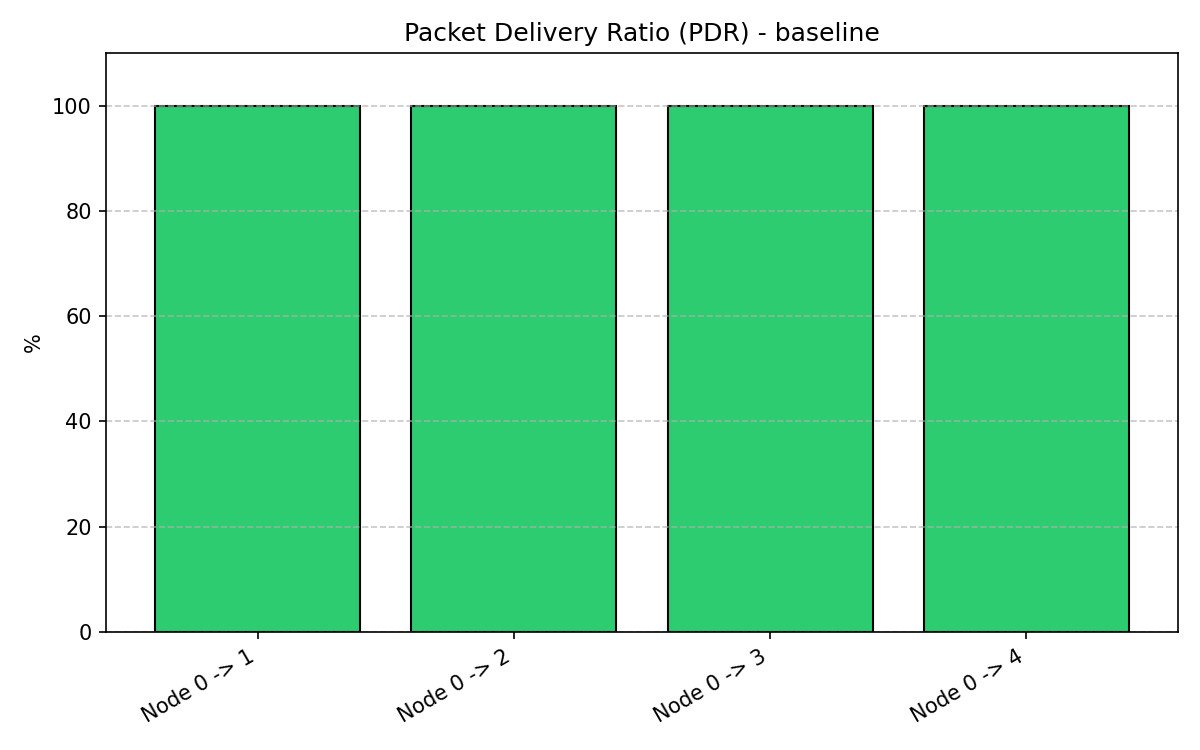
\includegraphics[width=0.7\textwidth]{./img/baseline_pdr.png}
		\caption{نمودار Packet Delivery Ratio در سناریوی baseline}
		\label{fig:baseline-pdr}
	\end{figure}
	
	در این شرایط ایده‌آل و غیراشباع، نرخ تحویل بسته (PDR) برای تمامی گره‌ها دقیقاً ۱۰۰ درصد است (شکل \ref{fig:baseline-pdr}) و مسیریابی RIP و انتقال MAC بدون از دست رفتن بسته‌ها انجام شده است؛ این نتیجه نشان می‌دهد که در بار سبک، نه ازدحام MAC و نه محدودیت همگرایی RIP، هیچ‌کدام مانعی برای تحویل کامل ترافیک ایجاد نمی‌کنند.
	
	\subsection{سناریوی ترافیک سنگین \lr{(Heavy Traffic)}}
	
	در این سناریو نرخ تزریق ترافیک به‌شدت افزایش یافته تا شبکه به حالت اشباع (Saturation) برسد.
	
	\begin{figure}[H]
		\centering
		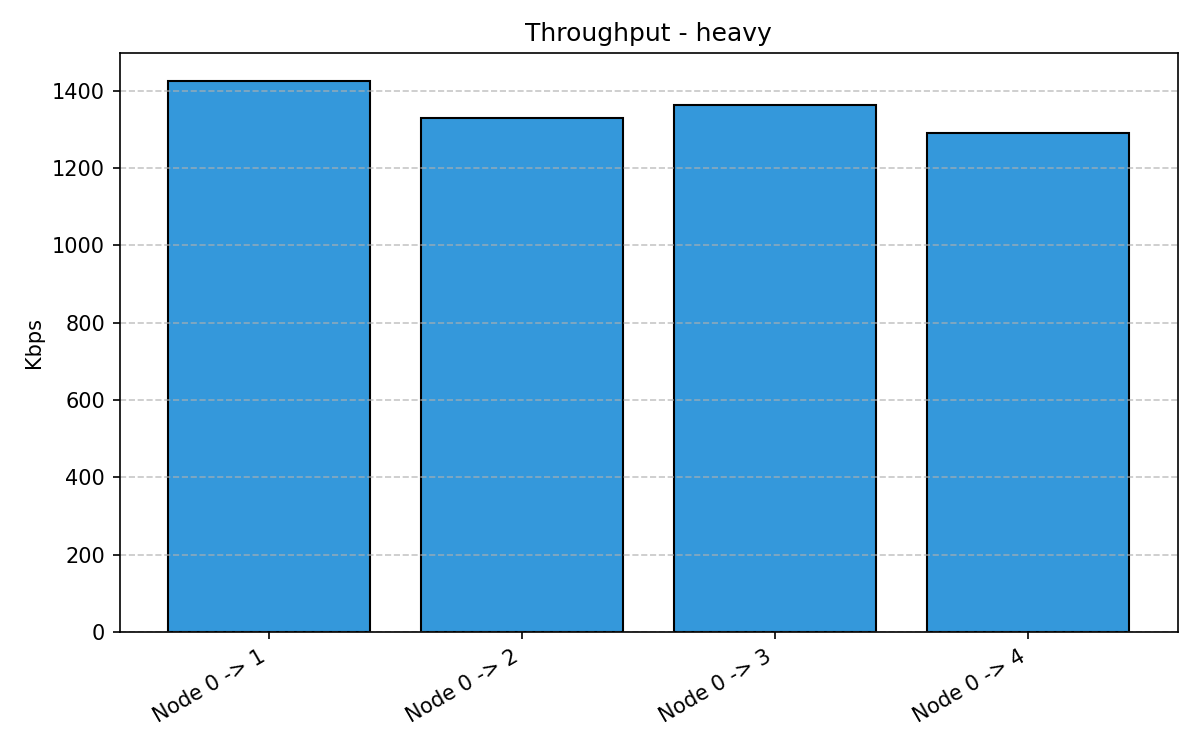
\includegraphics[width=0.7\textwidth]{./img/heavy_throughput.png}
		\caption{نمودار throughput در سناریوی ترافیک سنگین}
		\label{fig:heavy-throughput}
	\end{figure}
	
	در شکل \ref{fig:heavy-throughput} مشاهده می‌شود که throughput هر جریان روی مقداری بین ۱۳۰۰ تا ۱۴۰۰ کیلوبیت بر ثانیه متوقف شده است، به‌رغم این‌که نرخ تزریق درخواستی به‌مراتب بالاتر از این مقدار است. این سقف، نمایانگر ظرفیت مؤثر 
	\lr{(Effective Capacity)} 
	کانال \lr{802.11b} در این توپولوژی چندگامی است؛ این مقدار به‌طور قابل‌توجهی پایین‌تر از نرخ نظری فیزیکی ۱۱ مگابیت بر ثانیه است، چون باید بین چهار جریان هم‌زمان و چندین گام میانی تقسیم شود و سربار ناشی از DIFS، backoff، و ACK نیز از ظرفیت مفید کانال می‌کاهد. این پدیده نمونه‌ی کلاسیکی از پدیده‌ی شناخته‌شده‌ی «کاهش ظرفیت چندگامی»
	\lr{ (multi-hop capacity degradation)} 
	در شبکه‌های بی‌سیم ad-hoc است، که طبق آن ظرفیت end-to-end یک مسیر $h$‑گامی می‌تواند به نسبت تقریبی $1/h$ نسبت به ظرفیت یک‌گامی کاهش یابد، چون هر گام میانی هم باید بسته را دریافت و هم دوباره ارسال کند و این دو عمل بر سر همان کانال رادیویی مشترک رقابت می‌کنند.
	
	\begin{figure}[H]
		\centering
		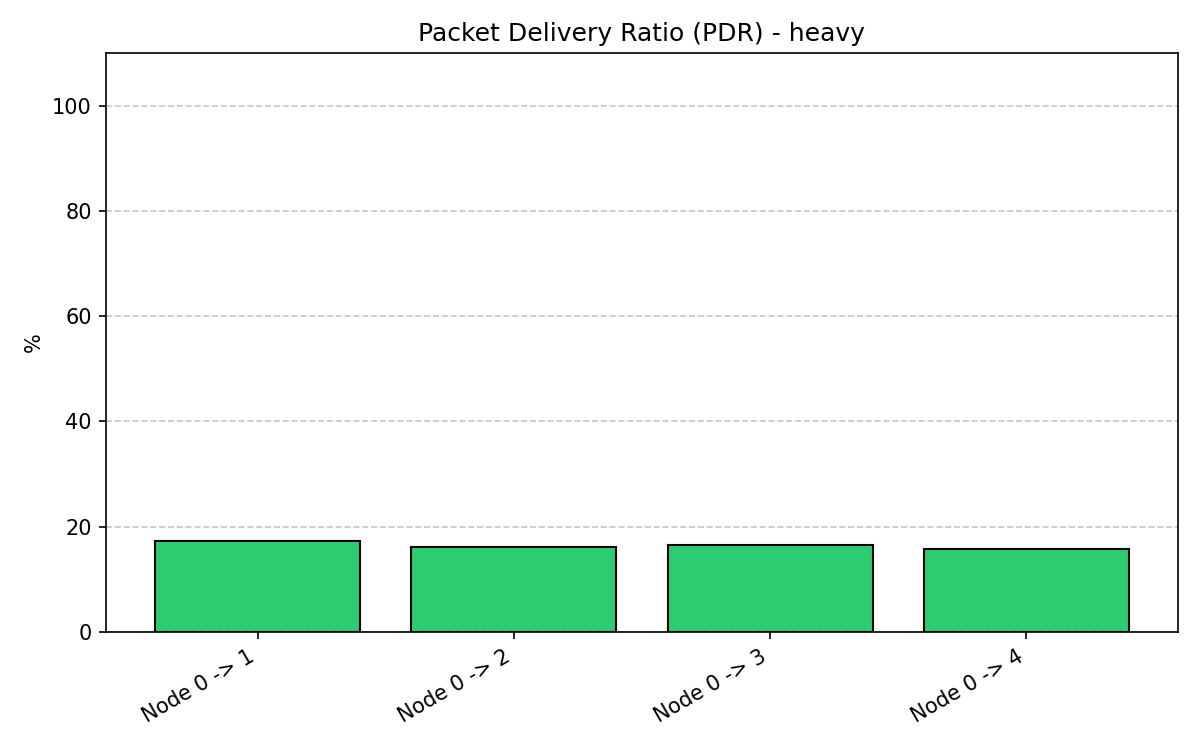
\includegraphics[width=0.85\textwidth]{./img/heavy_pdr.png}
		\caption{سقوط شدید Packet Delivery Ratio در سناریوی ترافیک سنگین}
		\label{fig:heavy-pdr}
	\end{figure}
	
	بارزترین خروجی این سناریو، سقوط شدید PDR به زیر ۲۰ درصد برای تمامی جریان‌هاست (شکل \ref{fig:heavy-pdr}). در توپولوژی خطی، ترافیک بالا باعث ایجاد تداخل شدید درون‌جریانی
	\lr{ (Intra-flow Interference)}
	 و بروز پدیده گره پنهان
	 \lr{ (Hidden Node Problem) }
	 می‌شود. مکانیزم عقب‌نشینی (Backoff) در CSMA/CA توانایی مدیریت این حجم از برخوردها را ندارد و بخش عمده‌ای از بسته‌ها به دلیل سرریز شدن صف‌های ارسال (تنظیم پیش‌فرض اندازه‌ی صف در NS-3 محدود است) یا پایان یافتن محدودیت تلاش مجدد MAC (که پس از تعداد مشخصی retransmission ناموفق، بسته را به‌طور کامل dropped می‌کند)، از بین می‌روند. این افت شدید PDR در کنار محدود ماندن throughput روی یک سقف ثابت، به‌خوبی نشان می‌دهد که اشباع کانال نه‌فقط باعث کاهش بازده، بلکه باعث اتلاف واقعی منابع شبکه (تلاش‌های ارسال ناموفق که خود نیز کانال را اشغال می‌کنند) نیز می‌شود.
	
	\subsection{سناریوی مقیاس‌پذیری (Scalability): افزایش تعداد گره‌ها}
	
	در این سناریو شبکه به ۱۵ گره در یک ساختار خطی گسترش یافته است تا محدودیت‌های پروتکل‌ها محک زده شود. نرخ ترافیک همان \lr{\texttt{500kbps}} است، یعنی بار سبک و قابل‌مدیریت برای CSMA/CA حفظ شده تا بتوان اثر افزایش قطر شبکه را به‌طور مجزا (بدون آلودگی با اثر اشباع کانال) بررسی کرد.
	
	\begin{figure}[H]
		\centering
		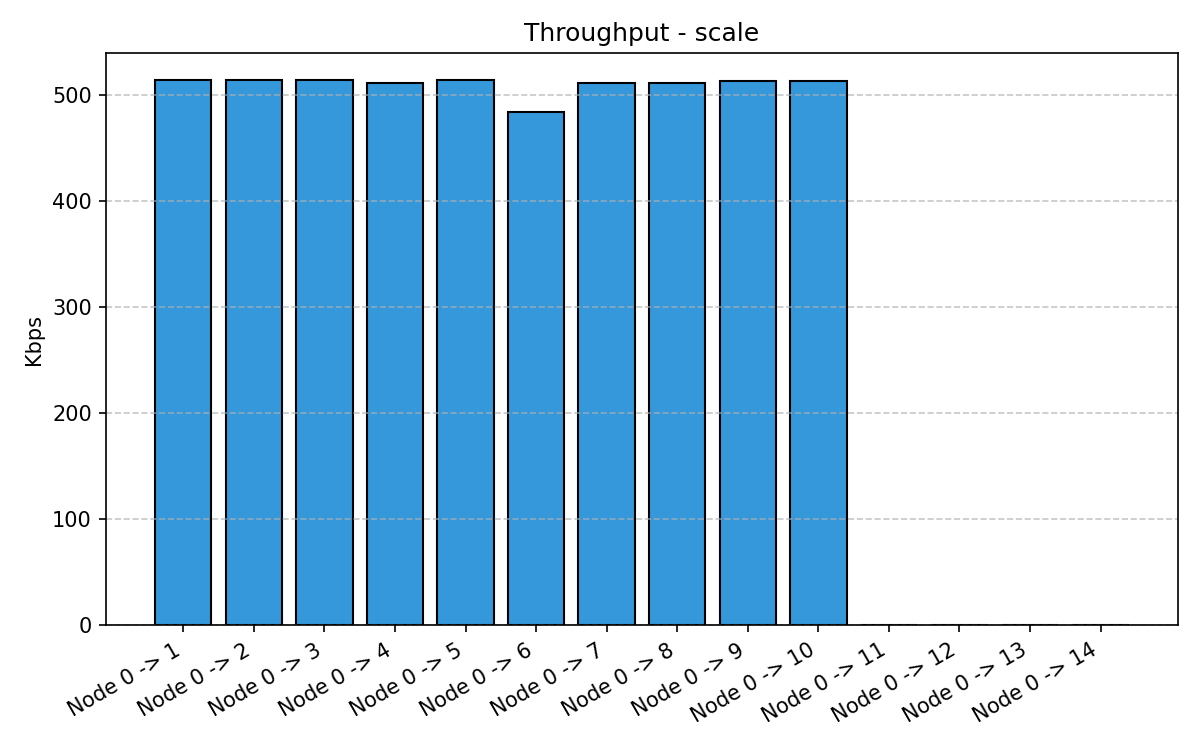
\includegraphics[width=0.85\textwidth]{./img/scale_throughput.png}
		\caption{صفر شدن Throughput گره‌های انتهایی در سناریوی مقیاس‌پذیری}
		\label{fig:scale-throughput}
	\end{figure}
	
	\begin{figure}[H]
		\centering
		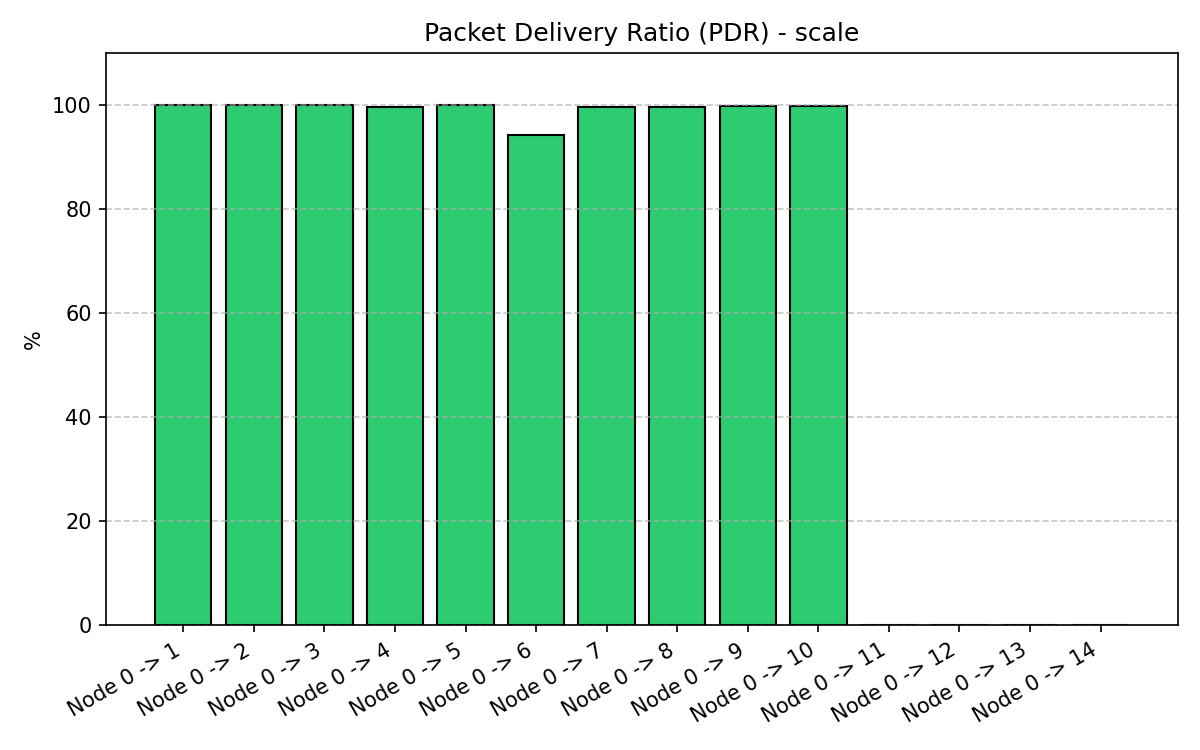
\includegraphics[width=0.85\textwidth]{./img/scale_pdr.png}
		\caption{تغییرات PDR و قطع ارتباط گره‌های دورتر در سناریوی مقیاس‌پذیری}
		\label{fig:scale-pdr}
	\end{figure}
	
	برخلاف تئوری افت یکنواخت پهنای باند، نمودارهای \ref{fig:scale-throughput} و \ref{fig:scale-pdr} یک نقطه ضعف بنیادین در پروتکل RIP را آشکار می‌کنند، نه یک افت تدریجی ناشی از تداخل MAC. گره‌های ۱ تا ۱۰ توانسته‌اند ترافیک خود را با PDR نزدیک به ۱۰۰٪ دریافت کنند (با یک افت جزئی در گره ۶ که به‌عنوان تنگنا یا Bottleneck میانی زنجیره عمل کرده است، چون این گره باید هم‌زمان نقش بازپخش (relay) برای ترافیک گره‌های دورتر را ایفا کند و هم ترافیک خودش را دریافت کند). اما PDR و Throughput برای گره‌های ۱۱ تا ۱۴ کاملاً صفر است؛ این یک افت ناگهانی (cliff-edge) است، نه یک کاهش تدریجی.
	
	دلیل این امر، زمان طولانی همگرایی (Convergence Time) در پروتکل RIP است. انتشار دوره‌ای جداول مسیریابی در یک زنجیره‌ی طولانی به زمان بسیار زیادی نیاز دارد، چون اطلاع‌رسانی یک مسیر جدید باید گام‌به‌گام تا انتهای زنجیره منتشر شود و در هر گام، علاوه‌بر تأخیر انتشار، باید منتظر دوره‌ی بعدی broadcast دوره‌ای RIP نیز ماند. در نتیجه، پیش از پایان یافتن فاصله‌ی زمانی اختصاص‌یافته برای همگرایی، RIP فرصت نکرده مسیر معتبری برای گره‌های انتهایی (۱۱ تا ۱۴) پیدا کند. در نتیجه، بسته‌های مربوط به این گره‌ها به‌دلیل نداشتن مسیر (\lr{No Route to Host}) همان در گره مبدأ (یا اولین گره‌ی میانی فاقد مسیر) دراپ شده‌اند، بدون این‌که حتی فرصتی برای ورود به رقابت MAC داشته باشند. این نتیجه به‌روشنی نشان می‌دهد که در این سناریوی خاص، گلوگاه عملکرد، لایه‌ی شبکه (RIP) است، نه لایه‌ی MAC.
	
	\subsection{مقایسه‌ی تطبیقی سه سناریو}
	
	\begin{table}[H]
		\centering
		\caption{جمع‌بندی مقایسه‌ای کیفی سه سناریوی شبیه‌سازی‌شده}
		\begin{tabular}{lccc}
			\toprule
			معیار & Baseline & Heavy Traffic & Scalability \\
			\midrule
			تعداد گره‌ها & ۵ & ۵ & ۱۵ \\
			نرخ هر جریان & \lr{500kbps} & اشباع‌کننده & \lr{500kbps} \\
			وضعیت کانال & غیراشباع & اشباع‌شده & غیراشباع برای نودهای ابتدایی \\
			throughput & تحویل کامل & محدود به ظرفیت عملی & صفر برای نودهای انتهایی \\
			تأخیر متوسط & پله‌ای (وابسته به گام) & بسیار بالا & پله‌ای افزایشی \\
			PDR & ۱۰۰٪ & افت شدید (زیر ۲۰٪) & ۱۰۰٪ برای همسایگان، ۰٪ برای دوردست \\
			چالش اصلی & - & Hidden Node و تداخل MAC & کندی همگرایی RIP \\
			\bottomrule
		\end{tabular}
	\end{table}
	
	این جدول به‌خوبی نشان می‌دهد که علت اصلی افت عملکرد در هر سناریو کاملاً متفاوت است: در heavy traffic، گلوگاه در لایه‌ی MAC و ظرفیت فیزیکی کانال است؛ در حالی‌که در scalability، گلوگاه در لایه‌ی شبکه و سرعت محدود پروتکل مسیریابی distance-vector است. این تفکیک علت‌ها، اهمیت طراحی آزمایش با کنترل دقیق متغیرها (تغییر یک پارامتر در هر سناریو، با ثابت نگه‌داشتن بقیه) را نشان می‌دهد.
	

	\section{پاسخ به سوالات پروژه}
	
	\subsection{چگونگی مدیریت ارسال‌های هم‌زمان توسط CSMA/CA و دلیل برتری آن نسبت به CSMA/CD در محیط بی‌سیم}
	
	CSMA/CA با استفاده از مکانیزم DCF، ارسال هم‌زمان را با ترکیبی از حس‌کردن کانال پیش از ارسال 
	\lr{(Carrier Sense)}
	، فاصله‌ی زمانی اجباری DIFS، و backoff تصادفی از یک Contention Window مدیریت می‌کند؛ هر گره پیش از ارسال باید کانال را برای مدت DIFS آزاد ببیند و سپس یک تایمر backoff تصادفی را شمارش معکوس کند که در صورت مشغول‌شدن کانال در میانه‌ی راه، متوقف (freeze) و پس از آزاد شدن مجدد کانال ادامه می‌یابد. در نتایج این پروژه، این مکانیزم در سناریوی baseline به‌خوبی توانست چهار جریان هم‌زمان را بدون افت PDR مدیریت کند (\lr{PDR }صد درصد)، اما در سناریوی heavy traffic که نرخ ترافیک از ظرفیت مؤثر کانال فراتر رفت، backoff نمایی توانست throughput را روی یک سقف نسبتاً پایدار نگه دارد، هرچند با هزینه‌ی افت شدید PDR و افزایش چشمگیر تأخیر.
	
	دلیل برتری CSMA/CA نسبت به CSMA/CD در محیط بی‌سیم، به دو محدودیت فیزیکی بنیادین بازمی‌گردد. نخست، رادیوهای معمولی Wi-Fi به‌صورت half-duplex عمل می‌کنند و توان سیگنال ارسالی یک گره به‌مراتب از توان سیگنال دریافتی است؛ بنابراین گیرنده‌ی همان گره عملاً قادر به تشخیص یک تداخل ضعیف از سوی گره‌ی دیگر در حین ارسال خودش نیست (سیگنال خودش signal دریافتی‌های دیگر را می‌پوشاند). دوم، مسئله‌ی hidden terminal باعث می‌شود دو گره که هر دو در محدوده‌ی یک گیرنده‌ی مشترک هستند، اما خودشان از محدوده‌ی رادیویی یکدیگر خارج باشند، اصلاً از ارسال هم‌زمان یکدیگر مطلع نشوند. این دو محدودیت در شبکه‌های سیمی (که در آن‌ها CSMA/CD کاربرد دارد) به‌دلیل ساختار اشتراکی و متقارن کابل وجود ندارند. به همین دلیل، \lr{802.11} به‌جای رویکرد «تشخیص پس از وقوع» 
	\lr{(Collision Detection)}،
	 رویکرد «پیشگیری پیش از وقوع» 
	\lr{ (Collision Avoidance)} 
	 را برگزیده و از مکانیزم تأییدیه‌ی صریح (ACK) برای جبران ناتوانی در تشخیص مستقیم collision استفاده می‌کند.
	
	\subsection{مسیرهای کشف‌شده توسط RIP و سرعت برقراری آن‌ها}
	
	با توجه به توپولوژی خطی به‌کاررفته در این پروژه، RIP مسیرهایی متناظر با زنجیره‌ی گام‌به‌گام بین گره‌ها کشف کرده است: برای رسیدن از گره ۰ به گره $k$، مسیر بهینه (و در این توپولوژی، تنها مسیر ممکن) از طریق گره‌های میانی $1, 2, \dots, k-1$ عبور می‌کند، چون این توپولوژی برخلاف یک grid کامل، فاقد مسیرهای جایگزین 
	\lr{(alternate paths)} 
	است. الگوریتم Bellman-Ford توزیع‌شده‌ی RIP این مسیرها را با تبادل دوره‌ای بردارهای فاصله بین همسایگان مستقیم کشف می‌کند: هر گره فاصله‌ی خود تا هر مقصد را به همسایگانش اعلام می‌کند و همسایه این فاصله را به‌علاوه‌ی یک گام در نظر می‌گیرد.
	
	سرعت برقراری این مسیرها مستقیماً به قطر شبکه وابسته است. در سناریوی baseline با ۵ گره (قطر ۴ گام)، فاصله‌ی ۳۴ثانیه‌ای پیش از شروع ترافیک داده برای همگرایی کامل کافی بوده و نتیجه‌ی آن PDR صد درصد برای تمام جریان‌ها بوده است؛ این نشان می‌دهد که RIP در این مقیاس کوچک، طی چند دور تبادل پیام (به مراتب کمتر از زمان اختصاص‌یافته) به همگرایی کامل رسیده است. اما در سناریوی scalability با ۱۵ گره (قطر ۱۴ گام)، همان فاصله‌ی زمانی برای همگرایی کافی نبوده است: نتایج نشان می‌دهند که مسیرهای گره‌های ۱ تا ۱۰ به‌درستی برقرار شده‌اند (با PDR نزدیک به ۱۰۰٪)، اما مسیرهای گره‌های ۱۱ تا ۱۴ هرگز در جداول مسیریابی برقرار نشدند (PDR صفر) و بسته‌های مربوط به آن‌ها به‌دلیل «عدم وجود مسیر» در همان گره‌ی مبدأ یا نزدیک به آن دراپ شدند. این رفتار به‌وضوح نشان‌دهنده‌ی رابطه‌ی غیرخطی بین قطر شبکه و زمان همگرایی RIP است که در شبکه‌های بزرگ‌تر می‌تواند به یک محدودیت اساسی تبدیل شود.
	
	\subsection{تفاوت عملکرد بین چهار جریان ترافیکی}
	
	در سناریوی baseline، چهار جریان ترافیکی (به سمت گره‌های ۱ تا ۴) تفاوت معناداری در throughput و PDR نشان نمی‌دهند؛ همگی به throughput نزدیک به نرخ نامی ۵۰۰ کیلوبیت بر ثانیه و PDR صد درصد می‌رسند، چون بار کلی کانال هنوز در محدوده‌ی غیراشباع قرار دارد. اما تفاوت اصلی و سیستماتیک بین این چهار جریان، در معیار تأخیر end-to-end ظاهر می‌شود: تأخیر با تعداد گام‌های لازم برای رسیدن به هر مقصد، به‌صورت تقریباً خطی افزایش می‌یابد. جریان به‌سمت گره ۱ (تک‌گامی) کمترین تأخیر (حدود ۱ میلی‌ثانیه) و جریان به‌سمت گره ۴ (چهارگامی) بیشترین تأخیر (حدود ۵.۵ میلی‌ثانیه) را دارد، چون هر گام میانی، تأخیر صف‌بندی و رقابت MAC مستقل خود را به تأخیر تجمعی اضافه می‌کند. در سناریوی heavy traffic، این تفاوت به‌مراتب تشدید می‌شود، چون با اشباع کانال، تأخیر صف‌بندی در هر گام به‌طور نمایی (نه خطی) افزایش می‌یابد و جریان‌های با گام بیشتر، احتمال بیشتری برای drop شدن بسته‌هایشان در گره‌های میانی دارند، نه فقط در گام نهایی.
	
	\subsection{رفتار شبکه با تعداد گره‌ی بیشتر یا ترافیک سنگین‌تر}
	
	با افزایش حجم ترافیک (سناریوی heavy traffic)، شبکه به نقطه‌ی اشباع کانال می‌رسد: throughput تجمعی روی یک سقف ثابت (ظرفیت مؤثر کانال \lr{802.11b} در این توپولوژی چندگامی، که به‌مراتب کمتر از نرخ نظری ۱۱ مگابیت بر ثانیه است) متوقف می‌شود، در حالی‌که PDR به‌شدت سقوط می‌کند (به زیر ۲۰٪)، چون مکانیزم backoff نمایی دیگر قادر به مدیریت حجم بالای رقابت نیست و درصد بالایی از بسته‌ها پس از اتمام تلاش‌های مجدد مجاز، به‌طور کامل از بین می‌روند. این رفتار نشان‌دهنده‌ی فروپاشی کارایی 
	\lr{(performance collapse)}
	 معمول در شبکه‌های CSMA تحت بار بیش از ظرفیت است.
	
	با افزایش تعداد گره‌ها در یک نرخ ترافیک ثابت و سبک (سناریوی \lr{scalability})، اما رفتار شبکه به‌طور کیفی متفاوت است: گلوگاه دیگر MAC نیست، بلکه سرعت همگرایی RIP است. گره‌های نزدیک به مبدأ، عملکرد کامل (PDR ۱۰۰٪) را حفظ می‌کنند، اما از یک نقطه‌ی مشخص به بعد (در این پروژه، حدود گام دهم تا یازدهم)، PDR به‌طور ناگهانی به صفر سقوط می‌کند، نه به‌صورت تدریجی. این یک افت آستانه‌ای 
	\lr{(threshold effect)} 
	است، نه یک کاهش پیوسته، و علت آن کاملاً متفاوت از علت افت در سناریوی heavy traffic است.
	
	\subsection{محدودیت‌های احتمالی RIP و CSMA/CA در مقیاس بزرگ‌تر}
	
	محدودیت‌های RIP در مقیاس بزرگ شامل موارد زیر است: نخست، سرعت همگرایی کند که با قطر شبکه به‌صورت خطی (و در عمل، به‌دلیل وابستگی به دوره‌ی broadcast ثابت، حتی کندتر) افزایش می‌یابد؛ نتایج این پروژه دقیقاً همین محدودیت را برای شبکه‌ای با قطر ۱۴ گام نشان داد. دوم، محدودیت hop-count برابر ۱۶ به‌عنوان «بی‌نهایت»، که سقفی برای حداکثر قطر شبکه‌ی قابل‌پشتیبانی توسط RIP تحمیل می‌کند؛ شبکه‌هایی با قطر بیشتر از ۱۵ گام اساساً قابل مسیریابی صحیح با RIP نیستند. سوم، مشکل count-to-infinity در صورت قطع لینک، که می‌تواند زمان همگرایی مجدد پس از یک تغییر توپولوژی را به‌طور چشمگیری افزایش دهد. این محدودیت‌ها به‌طور کلی RIP را برای شبکه‌های ad-hoc بزرگ یا با تغییرات توپولوژیکی مکرر، نامناسب می‌سازند و استفاده از پروتکل‌های link-state (مانند OSPF) یا پروتکل‌های مخصوص شبکه‌های ad-hoc (مانند AODV یا OLSR، که برای مقابله با تحرک و تغییرات سریع توپولوژی طراحی شده‌اند) را در مقیاس بزرگ‌تر توجیه می‌کند.
	
	محدودیت‌های CSMA/CA در مقیاس بزرگ‌تر عمدتاً حول مسئله‌ی ظرفیت ثابت کانال مشترک می‌چرخد: با افزایش تعداد گره‌هایی که هم‌زمان در محدوده‌ی رادیویی یکدیگر قرار دارند یا با افزایش تعداد جریان‌های هم‌زمان از یک گره (مانند طراحی این پروژه که گره صفر باید با تمام گره‌های دیگر هم‌زمان ارتباط برقرار کند)، رقابت بر سر کانال به‌صورت نمایی افزایش می‌یابد و throughput عادلانه 
	\lr{(fair throughput)}
	 به ازای هر جریان کاهش می‌یابد؛ این پدیده با نتایج heavy traffic در این پروژه به‌خوبی نشان داده شد. علاوه‌بر این، در توپولوژی‌های چندگامی بزرگ‌تر، مسئله‌ی hidden terminal با افزایش تعداد گره‌ها تشدید می‌شود، چون احتمال وجود جفت‌گره‌هایی که هم‌زمان در محدوده‌ی یک گیرنده‌ی مشترک باشند اما خارج از محدوده‌ی شنیداری یکدیگر باشند، با اندازه‌ی شبکه افزایش می‌یابد. در نهایت، هر گام میانی در یک مسیر طولانی، علاوه‌بر تحمیل تأخیر تجمعی (که در نتایج baseline این پروژه به‌وضوح دیده شد)، عملاً ظرفیت کانال را نیز با خود ارسال (relay) بیشتر مصرف می‌کند که به کاهش ظرفیت end-to-end با نسبت تقریبی $1/h$ منجر می‌شود، که هر دو محدودیت RIP و CSMA/CA با افزایش مقیاس شبکه، به‌طور هم‌زمان و تشدیدکننده‌ی یکدیگر عمل می‌کنند.
	
	\vfill
	\begin{flushleft}
		\Huge\textbf{مرسی از توجه شما}
	\end{flushleft}
	
\end{document}